\RequirePackage{filecontents}
\begin{filecontents}{mybibliography.bib}
@misc{rehfeld,
	AUTHOR = "Stephan Rehfeld",
	TITLE = "{Digitale Bilder}",
	HOWPUBLISHED = "{\url{https://public.beuth-hochschule.de/~rehfeld/lehre/2015/ss/digitale-bilder.pdf}}",
	YEAR = "{2015}"
}

@article{drepper2007every,
  title={What every programmer should know about memory},
  author={Drepper, Ulrich},
  journal={Red Hat, Inc},
  volume={11},
  year={2007}
}

@online{big-o,
  title={Know Thy Complexities!},
  author={Eric Rowell},
  howpublished={\url{http://bigocheatsheet.com/}},
  year={2013}
}

\end{filecontents}	

\documentclass[tog]{acmsiggraph}

%%% Make the ``BibTeX'' word pretty...

\def\BibTeX{{\rm B\kern-.05em{\sc i\kern-.025em b}\kern-.08em
   T\kern-.1667em\lower.7ex\hbox{E}\kern-.125emX}}

% fürs  code highlighting
\usepackage{listings}

% für hyperlinks http://en.wikibooks.org/wiki/LaTeX/Hyperlinks
\usepackage{hyperref}

% für korrkte Umlaute
\usepackage[utf8]{inputenc}

% für Umlaute
% \usepackage[T1]{fontenc}\usepackage{lmodern}

% für Verweise
\usepackage{cite}

% für korrekte mathematische Zeichen
\usepackage{amsfonts}

% für deutsche Silbentrennung
\usepackage[ngerman]{babel}

% deutsche anführungen
\usepackage[autostyle]{csquotes}


%%% Used by the ``review'' variation; the online ID will be printed on 
%%% every page of the content.

\TOGonlineid{45678}

%%% Used by the ``preprint'' variation.

\TOGvolume{0}
\TOGnumber{0}

\title{Digitale Bilder}

\author{Reguieg, Ibrahim Khaled
\and Döring, Jules}
\pdfauthor{Reguieg, Döring}

\keywords{Digitale Bilder, Bildverarbeitung, CG1 }

\begin{document}

%%% This is the ``teaser'' command, which puts an figure, centered, below 
%%% the title and author information, and above the body of the content.

 \teaser{
   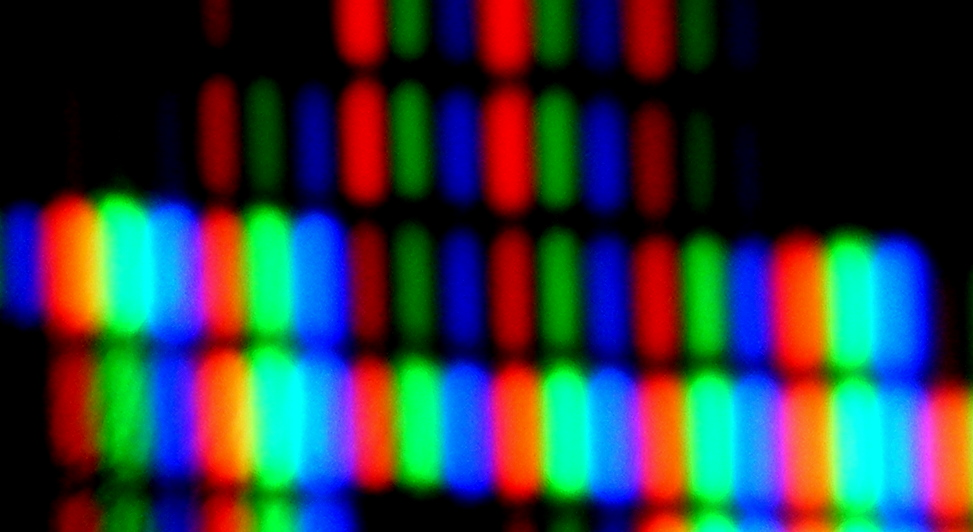
\includegraphics[width=7in, trim=13mm 30mm 8mm 100mm, clip=true]{images/Jeffrey_Smith_Flikr_CC-BY-ND-2-0.jpg}
   \caption{\href{https://www.flickr.com/photos/jmsmith000/3097202394}{Jeffrey Smith 2008 }}
 }

\maketitle



\begin{abstract}
In dieser Mitschrift wird beschrieben, wie digitale Bilder im Rechner dargestellt werden.
In der Realität werden Bilder durch reflektiertes Licht erzeugt.
Das führt zu den folgenden Fragestellungen:

"`Wie stellen wir Farben und Bilder am Computer dar?\,"'

"`Wie werden Bilder im Computer repräsentiert?\,"'

Hier soll ein Weg hergeleitet werden, Bilder in einer Form zu abstrahieren, mit der Computerprogramme effizient arbeiten können.
\end{abstract}

\section{Was ist ein Bild?}

Bilder sind stetig. Stetige Bilder sind allerdings kaum im Computer darstellbar, da dieser mit diskreten Werten arbeitet. Also müssen wir die stetigen Bilder in diskrete Bilder umwandeln.

\subsection{Formal Mathematisch}
Am besten dafür eignet sich die folgende stetige mathematische Funktion, die die Menge der Koordinaten R auf die Menge der Farben V abbildet:
\begin{equation}\label{eq:eins}I(x,y): R \rightarrow V\end{equation}

Die Funktion (\ref{eq:eins}) bildet die Menge der Koordinaten auf die Menge der Farben ab.

\begin{equation}\label{eq:two}R\subset \mathbb{R}^2\end{equation}

(\ref{eq:two}) besagt, dass die Farben R eine Teilmenge des  kartesischen Produktes  $\mathbb{R}$ x $\mathbb{R}$

\begin{equation}\label{eq:three}V = \mathbb{R}^+ \: Graustufenbild\end{equation}

(\ref{eq:three}) Der Farbraum für ein Fraustufenbild entspricht den positiven reellen Zahlen.

\begin{equation}\label{eq:four}V = \left (\mathbb{R}^+  \right )^3 \: Farbbild\end{equation}

(\ref{eq:four}) Für eine Farbbild wird der Farbraum dem dreidimensionalen positiven Raum zugewiesen.


Diese Art der Modellierung ist unnötig genau. Durch optische Ungenauigkeiten, denen die menschliche Wahrnehmung unterliegt, findet eine sehr viel gröbere Abtastung statt. Diese kann man zur Vereinfachung des Modells nutzen.

\subsection{Wahrnehmung bei Menschen}
Je weiter ein Objekt entfernt ist, um so kleiner ist die Abbildung auf die Stäbchen und Zapfen unserer Netzhaut, da das Licht von mehreren Punkten des gesehenen Objekts auf einen Punkt auf der Netzhaut projiziert wird. Ist ein Objekt sehr nahe, wie bei \ref{fig:Objekt nah am Auge} wird es deutlich auf den Zellen der Netzhaut abgebildet.

\begin{figure}[ht]
  \centering
  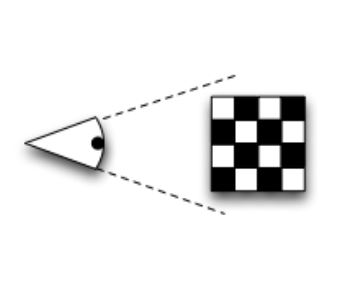
\includegraphics[width=.75in]{images/AugeObjektNah}
  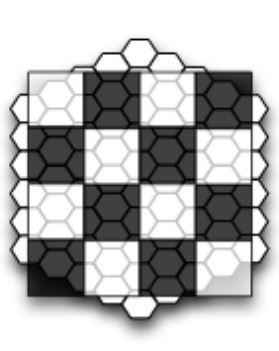
\includegraphics[width=0.5in]{images/SinneszelleObjektNah}
  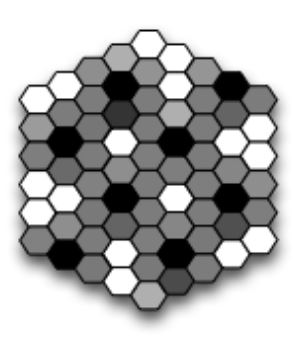
\includegraphics[width=0.5in]{images/AbbildungAufSinneszelleObjektNah}
  \caption{Objekt nah am Auge.}
  \label{fig:Objekt nah am Auge}
  \cite{rehfeld}
\end{figure}

 Somit hat das menschliche Auge, wie bei \ref{fig:Objekt fern vom Auge} keine Chance mehr die Unterschiede zwischen nahegelegenen Punkten wahrzunehmen.

\begin{figure}[ht]
  \centering
  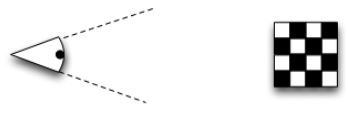
\includegraphics[width=1.5in]{images/AugeObjektFern}
  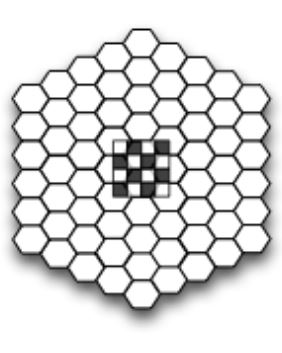
\includegraphics[width=0.5in]{images/SinneszelleObjektFern}
  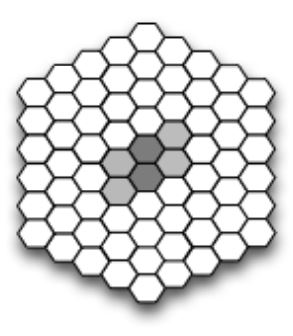
\includegraphics[width=0.55in]{images/AbbildungAufSinneszelleObjektFern}
  \caption{Objekt fern vom Auge}
  \label{fig:Objekt fern vom Auge}
  \cite{rehfeld}
\end{figure}

Auch beim Druck findet dieses Begebenheit Anwendung, beispielsweise druckt der Druckkopf ganz kleine Muster, um aus Gelb und Magenta Rot oder Orange zu mischen, wie auf Abbildung \ref{fig:Aus Grundfarben wird neue eine Farbe} zu sehen ist.

\begin{figure}[ht]
  \centering
  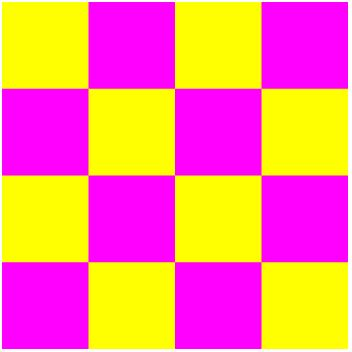
\includegraphics[width=0.5in]{images/gelbMagentaMusterGrob}
  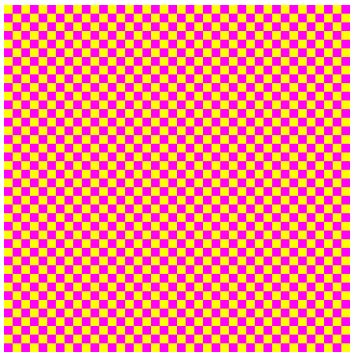
\includegraphics[width=0.5in]{images/gelbMagentaMusterFeiner}
  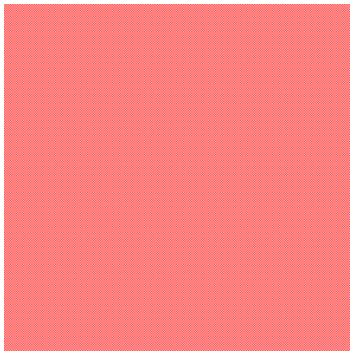
\includegraphics[width=0.5in]{images/gelbMagentaMusterFein}
  \caption{Farben mischen aus CMYK.}
  \label{fig:Aus Grundfarben wird neue eine Farbe}
  \cite{rehfeld}
\end{figure}

Ähnlich verhält es sich bei Bildschirmen, denn die mangelnde örtliche Auflösung führt zum Eindruck eines stetigen Bildes, wobei die Signale des Bildschirms eigentlich diskret sind.

\section{Umsetzung für Computer}
In diesem Abschnitt wird beschrieben, wie die Umsetzung der Bilder in er Programmierung aussehen.
Naheliegend ist es, ein Bildgitter durch einen zweidimensionalen \textit{byte} Array pro Farbkanal darzustellen.
Nun kann jeder Subpixel bearbeitet werden, indem wir mit zwei geschachtelten For-Schleifen über die Koordinaten iterieren und dort die RGB-Farbwerte setzen.
\begin{lstlisting}[caption=Bildgitter aus zweidimensionalen Byte Array pro Farbkanal]
final byte[][]pic = new byte[640][480][3];

for (int x = 0; x < width; ++x){
  for (int y = 0; y < height; ++y){
    byte r = pic [x][y][0];
    byte g = pic [x][y][1];
    byte b = pic [x][y][2];
    }
  }
\end{lstlisting}

\subsection{Optimierung für CPU Caching}

SRAM $\rightarrow$ ist \textit{teuer} aber \textit{schnell} \\
DRAM $\rightarrow$ ist \textit{günstig} aber \textit{langsam}

Auf der CPU befinden sich schnelle kleine SRAM basierte Speicher die als Caches benutzt werden. Cachecontroller versuchen zu errechnen auf welche Speicheradressen als nächstes zugegriffen wird und laden die Daten präventiv ins schnellere Cache. Dadurch muss die CPU seltener warten bis Daten aus dem langsamen Hauptspeicher auf DRAM Basis geladen sind.
Modernen CPUs haben üblicherweise drei Cache-Level mit denen man versucht die \textit{Cache Misses} zu minimieren.

\cite{drepper2007every}

\subsection{Graustufenbild}
Um \textit{Cacheprediction} besser aus zu nutzen ist es also sinnvoll, Daten hintereinander abzulegen. Der folgende Code ist ein Beispiel für ein Graustufenbild als eindimensionales Array.

\begin{lstlisting}[caption=Graustufenbild]
final byte[][] pic = new byte [width * height];

for (int x = 0; x < width; ++x) {
  for (int y = 0; y < height; ++y) {
    byte g = pic [y * width +x];
  }
}
\end{lstlisting}

\subsection{Farbbild mit separierten Kanälen}
Ähnlich kann man ein Farbbild modellieren, indem man die Farbkanäle einen nach dem anderen,wie in Abbildung XXX ablegt.

\begin{figure}[ht]
  \centering
  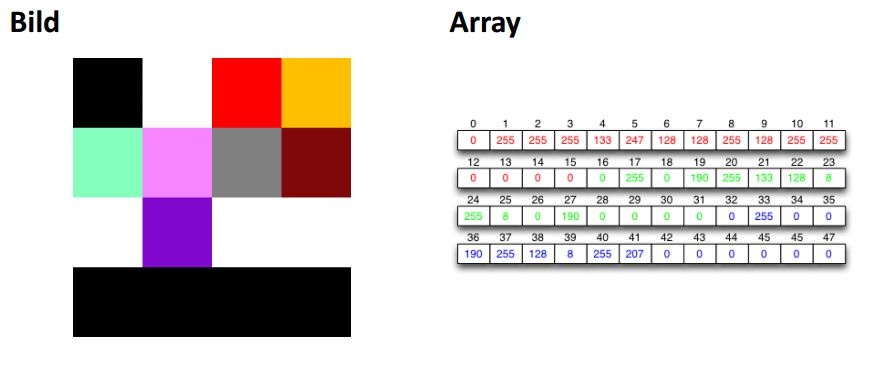
\includegraphics[width=2.0in]{images/BildKomponentenweise}
  \caption{Farbbild mit separierten Farbkanälen.}
  \label{fig:Separierte Farbkanaele}
  \cite{rehfeld}
\end{figure}

\begin{lstlisting}[caption=Farbbild mit separierten Kanälen]
final byte[][] pic = new byte [640 * 480 * 3];
SomeImageLoader.loadInto(pic);
for (int x = 0; x < width; ++x) {
  for (int y = 0; y < height; ++y) {
    final byte red = pic[0 * width * height
    + y * width + x ];
    
    final byte green = pic[1 * width * height 
    + y * width + x ];

    final byte blue = pic[2 * width * height
    + y * width + x ];
    }
  }
\end{lstlisting}

\subsection{Farbbild Pixelweise}
Eine weitere Möglichkeit besteht darin, jeden Pixel durch 3 aufeinander folgende Subpixel darzustellen.

\begin{lstlisting}[caption=Farbbild Pixelweise]
final byte[][] pic = new byte [640 * 480 * 3];

for (int x = 0; x < width; ++x){
  for (int y = 0 ; y < height; ++y){
    byte r = pic [y * width *3 + x*3 +0]; 
    byte g = pic [y * width *3 + x*3 +3];
    byte b = pic [y * width *3 + x*3 +2];
    }
  }
\end{lstlisting}

\subsection{Farbbild Pixelweise als Integer}
Die häufigste Darstellung ist allerdings die pixelweise Darstellung in einem Array vom Typ Integer, da sie mehrere Vorteile in sich vereint. Die Performanz wird einerseits durch \textit{Data structure alignment} auf Speicherseite und andererseits durch Ausnutzen hochperformanter Shiftoperationen für Subpixelzugriffe gewährleistet. Zudem erhält man für Menschen verhältnismäßig gut interpretierbare Werte. \cite{big-o}

Der Zugriff auf Subpixel findet mittels Bitmasken und Shiftoperationen statt.

\begin{lstlisting}[caption=Farbbild Pixelweise als Integer]
final int height = 480;
final int width = 640;
final int[] pic = new int[height * width ];
SomeImageLoader.loadInto( pic );
for(int y = 0; y < height; ++y ) {
  for(int x = 0; x < width; ++x ) {
    int red = (pic[ y * width + x ] &
    0xff0000) >> 16;
    int green = (pic[ y * width + x ] &
    0xff00) >> 8;
    int blue = pic[ y * width + x ] & 0xff;

    pic[y * width + x ] = 
    ((red & 0xff) << 16) | 
    ((green & 0xff) << 8) | 
    (blue & 0xff);
  }
}
\end{lstlisting}

\begin{figure}[ht]
  \centering
  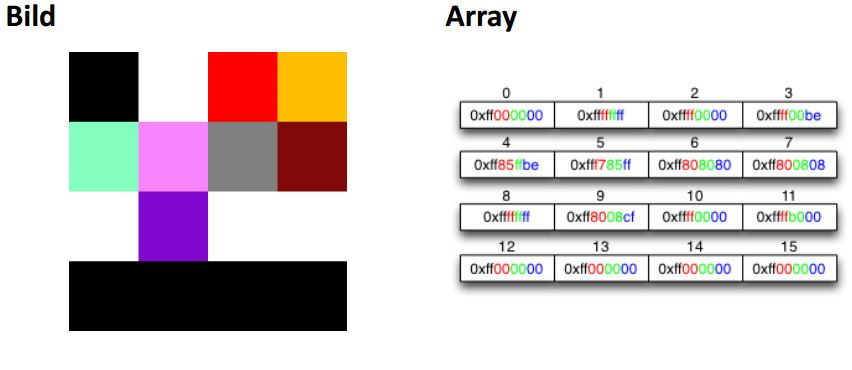
\includegraphics[width=2.0in]{images/BildPixelweiseInteger}
  \caption{Farbbild in pixelweiser Darstellung im Integer Array.}
  \label{fig:Pixelweise Darstellung im Array.}
  \cite{rehfeld}
\end{figure}


\section{Koordinatensystem}
Bei allen beschriebenen Vorgängen ist zu beachten, dass das in der Computergrafik übliche Koordinatensystem mathematisch korrekt unten links beginnt und sich nach oben und rechts ausbreitet.

\begin{figure}[ht]
  \centering
  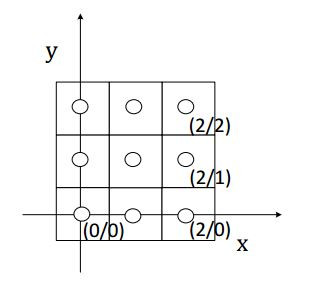
\includegraphics[width=1.0in]{images/koordinatenSystemComputergrafik}
  \caption{Bilder in der Computergrafik.}
  \label{fig:Koordinatenursprung unten links}
  \cite{rehfeld}
\end{figure}

In der Bildverarbeitung hingegen beginnt es gemäß der Leserichtung der westlichen Kultur sowie der Richtung in CRT Monitoren, oben links und breitet sich nach rechts und unten aus.
 
\begin{figure}[ht]
  \centering
  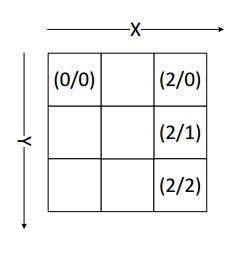
\includegraphics[width=1.0in]{images/koordinatenSystemBildverarbeitung}
  \caption{Bilder in der Bildverarbeitung.}
  \label{fig:Koordinatenursprung oben links}
  \cite{rehfeld}
\end{figure}


\bibliographystyle{acmsiggraph}
\nocite{*}
\bibliography{mybibliography}
\end{document}

